\chapter{Introduction}

   Real-world knowledge discovery processes typically consist
of complex data pre-processing, machine learning, evaluation,
and visualization steps. 
   Hence a data mining platform should allow complex nested 
operator chains or trees, provide transparent data handling, 
comfortable parameter handling and optimization, be flexible, 
extendable and easy-to-use.

   Depending on the task at hand, a user may want to interactively
explore different knowledge discovery chains and continuously 
inspect intermediate results, or he may want to perform highly 
automated data mining processes off-line in batch mode.
   Therefore an ideal data mining platform should offer both,
interactive and batch interfaces.

\rapidminer (formerly \textsc{Yale}) is an environment for machine learning and data mining processes. A modular operator
concept allows the design of complex nested operator chains for a huge number
of learning problems. The data handling is transparent to the operators. They
do not have to cope with the actual data format or different data views - the
\rapidminer core takes care of the necessary transformations. Today, \rapidminer is the 
world-wide leading open-source data mining solution and is widely used by
researchers and companies.

\rapidminer introduces new concepts of transparent data handling and process
modelling which eases process configuration for end users. Additionally
clear interfaces and a sort of scripting language based on XML turns \rapidminer
into an integrated developer environment for data mining and machine learning.
Some of these aspects will be discussed in the next sections. Please
refer to \cite{Mierswa/etal/2006a,Mierswa/etal/2003a,Ritthoff/etal/2001a} for further
explanations. We highly appreciate if you cite \rapidminer in your scientific work. 
Please do so by citing

\begin{quote}
Mierswa, I. and Wurst, M. and Klinkenberg, R. and Scholz, M. and Euler, T.,
\textsc{Yale} (now: \rapidminer): Rapid Prototyping for Complex Data Mining Tasks. In: Proceedings of the ACM SIGKDD
International Conference on Knowledge Discovery and Data Mining (KDD 2006), 2006.
\end{quote}


\section{\mbox{Modeling Knowledge Discovery} Processes as Operator Trees}

Knowledge discovery (KD) processes are often viewed as sequential 
operator chains.
   In many applications, flat linear operator chains are insufficient
to model the KD process and hence operator chains need to be nestable.
   For example a complex KD process containing a learning step, whose
parameters are optimized using an inner cross-validation, and which
as a whole is evaluated by an outer cross-validation.
   Nested operator chains are basically trees of operators.

In \rapidminer, the leafs in the operator tree of a KD process correspond
to simple steps in the modeled process.
   Inner nodes of the tree correspond to more complex or abstract
steps in the process.
   The root of the tree hence corresponds to the whole process.

   Operators define their expected inputs and delivered outputs
as well as their obligatory and optional parameters, which enables
\rapidminer to automatically check the nesting of the operators, the
types of the objects passed between the operators, and the 
mandatory parameters. This eases the design of complex data mining
processes and enables \rapidminer to automatically check the nesting of the 
operators, the types of the objects passed between the operators, 
and the mandatory parameters.


Figure~\ref{fig:methodvalidationchain_box} shows a nested KD process
for feature selection using a genetic algorithm with an inner cross-validation
for evaluating candidate feature sets and an outer cross-validation
for evaluating the genetic algorithm as a feature selector.


\begin{figure}[tbp]
  \center
  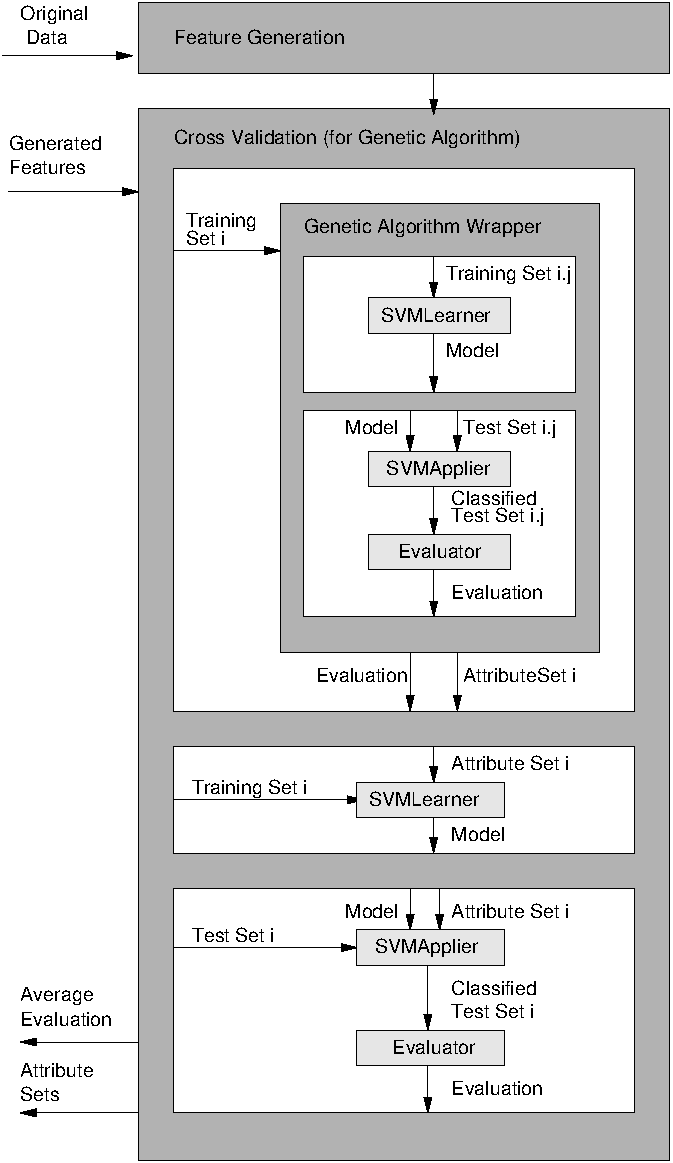
\includegraphics{graphics/genplusXValForGA.pdf}
  \caption[Feature selection using a genetic algorithm]{Nested operator chain for feature selection using a genetic algorithm.}
  \label{fig:methodvalidationchain_box}
\end{figure}





\section{\rapidminer as a Data Mining Interpreter}

\rapidminer uses XML (eXtensible Markup Language), a widely used language 
well suited for describing structured objects, to describe the
operator trees modeling KD processes.
   XML has become a standard format for data exchange.
Furthermore this format is easily readable by humans and machines. All
\rapidminer processes are described in an easy XML format. You can see this XML
description as a scripting language for data mining pocesses.

The graphical user interface and the XML based scripting language turn
\rapidminer into an IDE and interpreter for machine learning and data mining. Furthermore, the
XML process configuration files define a standardized interchange format
for data mining processes.




\section{Different Ways of Using \rapidminer}

\rapidminer can be started off-line, if the process configuration is provided
as XML file.
   Alternatively, the GUI of \rapidminer can be used to design the XML description
of the operator tree, to interactively control and inspect running processes, 
and to continuously monitor the visualization of the process results.
Break points can be used to check intermediate results and the data flow
between operators.
Of course you can also use \rapidminer from your program. Clear interfaces define an
easy way of applying single operators, operator chains, or complete operator
trees on you input data. A command line version and a Java API allows
invoking of \rapidminer from your programs without using the GUI. 
Since \rapidminer is entirely written in Java, it runs on any major
platform/operating system.




\section{Multi-Layered Data View Concept}
     

\rapidminer's most important characteristic is the ability to nest operator chains
and build complex operator trees. In order to support this characteristic the
\rapidminer data core acts like a data base management system and provides a
multi-layered data view concept on a central data table which underlies all
views. For example, the first view can select a subset of examples and the
second view can select a subset of features. The result is a single view which
reflects both views. Other views can create new attributes or filter the data
on the fly. The number of layered views is not limited.

This multi-layered view concept is also an efficient way to store different
views on the same data table. This is especially important for automatic data
preprocessing tasks like feature generation or selection. For example, the
population of an evolutionary operator might consist of several data views -
instead of several copies of parts of the data set. 
    
No matter whether a data set is stored in memory, in a file,
or in a database, \rapidminer internally uses a special type of data
table to represent it.
   In order not to unnecessarily copy the data set or subsets
of it, \rapidminer manages views on this table, so that only references
to the relevant parts of the table need to be copied or passed
between operators.
   These views are nestable as is for example required for nested
cross-validations by maintaining a stack of views.
   In case of an example set, views on the rows of the table 
correspond to subsets of the example set, and views on the
columns correspond to the selected features used to represent
these examples.




\section{Transparent Data Handling}

\rapidminer supports flexible process (re)arrangements which allows the search
for the best learning scheme and preprocessing for the data and learning task
at hand. The simple adaptation and evaluation of different process designs
allow the comparison of different solutions. 

\rapidminer achieves a transparent data handling by supporting several
types of data sources and hiding internal data transformations and
partitioning from the user. Due to the modular operator
concept often only one operator has to be replaced to evaluate its performance
while the rest of the process design remains the same. This is an important
feature for both scientific research and the optimization of real-world
applications.

The input objects of an operator may be consumed or passed on to 
following or enclosing operators. If the input objects are not required by
this operator, they are simply passed on, and may be used by later or outer 
operators.
This increases the flexibility of \rapidminer by easing the match of 
the interfaces of consecutive operators and allowing to pass objects
from one operator through several other operators to the goal operator.

Objects typically passed between operators are example sets, 
prediction models, evaluation vectors, etc.
Operators may add information to input objects, e.g. labels 
to previously unlabeled examples, or new features in a feature 
generation operator, and deliver these extended objects.




\section{Meta Data}

To guide the transformation of the feature space or the automatical search for
the best preprocessing, the user can define additional meta data on the data
set at hand. Meta data include the type of attributes or their unit (SI). This
information is for example used by the feature generation / construction
algorithms provided by \rapidminer. The definition of meta information on your data
is optional and if it is omitted \rapidminer tries to guess the correct data types.




\section{Large Number of Built-in Data Mining Operators}

\rapidminer provides more than 400 operators including:
\begin{description}
\item[Machine learning algorithms:] a huge number of learning schemes for
  regression and classification tasks including support vector machines (SVM),
  decision tree and rule learners, lazy learners, Bayesian learners, and
  Logistic learners. Several algorithms for association rule mining and
  clustering are also part of \rapidminer. Furthermore, we added several meta
  learning schemes including Bayesian Boosting.
\item[Weka operators:] all Weka operations like learning schemes and attribute
  evaluators of the Weka learning environment are also available and can be
  used like all other \rapidminer operators.
\item[Data preprocessing operators:] discretization, example and feature filtering,
  missing and infinite value replenishment, normalization, removal of useless
  features, sampling, dimensionality reduction, and more.
\item[Feature operators:] selection algorithms like forward selection,
  backward elimination, and several genetic algorithms, operators for feature
  extraction from time series, feature weighting, feature relevance, and
  generation of new features.
\item[Meta operators:] optimization operators for process design,
  e.g. example set iterations or several parameter optimization schemes.
\item[Performance evaluation:] cross-validation and other evaluation schemes,
  several performance criteria for classification and regression, operators
  for parameter optimization in enclosed operators or operator chains.
\item[Visualization:] operators for logging and presenting results. Create
  online 2D and 3D plots of your data, learned models and other process
  results.
\item[In- and output:] flexible operators for data in- and output, support of
several file formats including arff, C4.5, csv, bibtex, dBase, and reading
directly from databases.
\end{description}




\section{Extending \rapidminer}

\rapidminer supports the implementation of user-defined operators.
In order to implement an operator, the user simply needs to
define the expected inputs, the delivered outputs, the mandatory
and optional parameters, and the core functionality of the operator.
Everything else is done by \rapidminer. The operator description in XML
allows \rapidminer to automatically create corresponding GUI elements.
This is explained in detail in
chapter~\ref{sec:extending_rapidminer}. An easy-to-use plugin mechanism is provided
to add future operators or operators written by the \rapidminer community
into \rapidminer. Several plugins are already provided in the download
section of \rapidminer.

External programs can be integrated by implementing wrapper 
operators and can then be transparently used in any \rapidminer 
process.



\section{Example Applications}

\rapidminer has already been applied for machine learning and
knowledge discovery tasks in a number of domains including
feature generation and selection % to improve the classification and regression learning
\cite{Felske/etal/2003a,            %%  SFB-CI/C9-TR
      Klinkenberg/etal/2002a,       %%  FGML-2002
      Ritthoff/Klinkenberg/2003a,   %%  GECCO-2003
      Ritthoff/etal/2002b},         %%  UKCI-2002
concept drift handling
\cite{Klinkenberg/Joachims/2000a,   %%  ICML-2000
      Klinkenberg/2004a,
      Klinkenberg/2003a,
      Klinkenberg/Rueping/2003a},   %%  Daimler-WS-Buchkapitel
and transduction
\cite{Daniel/etal/2002a,            %%  SFB-CI-Ergebnisberichtbuchkapitel
      Klinkenberg/2001a}.           %%  IJCAI-2001-WS
In addition to the above-mentioned, current application domains of
\rapidminer also include
the pre-processing of and learning from time series
\cite{Mierswa/2004c,Mierswa/Morik/2005a,Mierswa/Morik/2005b},
meta learning \cite{Mierswa/Wurst/2005a,Mierswa/Wurst/2005b},
clustering, and text processing
and classification.  %% Word Vector Tool by Michael Wurst
There exist several plugins to provide operators for these special
learning tasks. Among these, there are some unusual plugins like GAStruct
which can be used to optimize the design layout for chemical plants
\cite{Mierswa/2005a,Mierswa/Geisbe/2004a}.


The Figures~\ref{fig:screen_experiment} and \ref{fig:screen_plot} 
show screenshots from two process definitions performed with the GUI version of \rapidminer.
   Figure~\ref{fig:screen_experiment} depicts the process tree and
the panel for setting the parameters of one of its operators in
a feature selection process using backward elimination as feature selector.
   Figure~\ref{fig:screen_plot} demonstrates the continuous result display
of a parameter optimization process.

\begin{figure}[ptbh]
  \center
    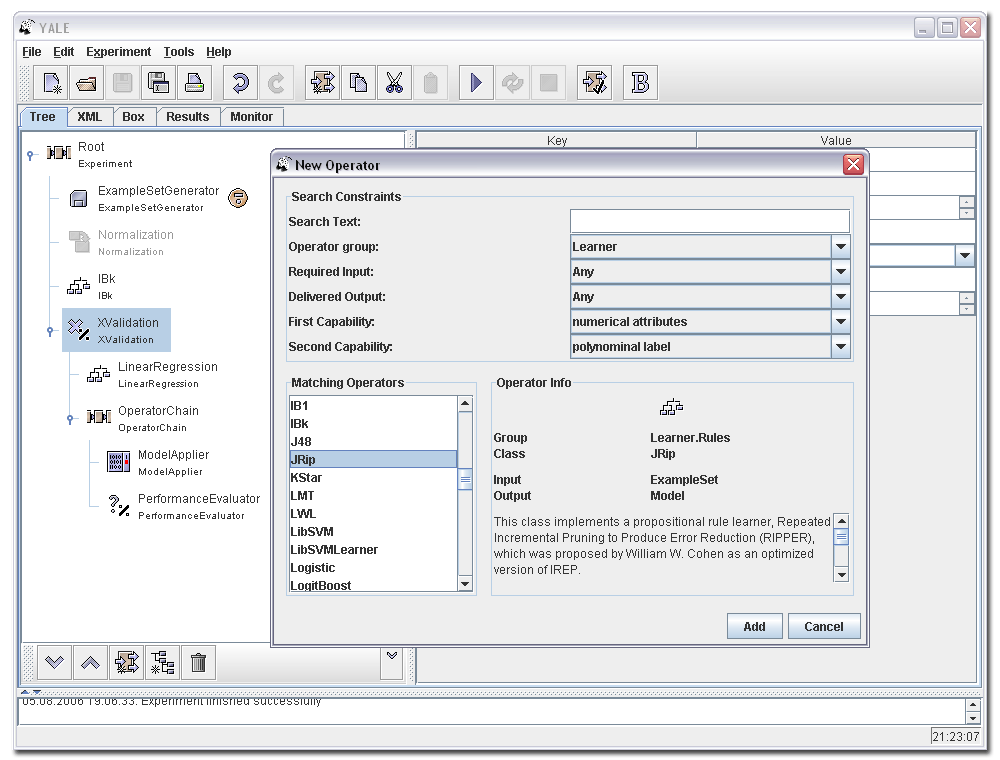
\includegraphics[height=0.4\textheight]{graphics/screenshots/screenshot_main1.png}
  \caption[\rapidminer GUI screenshot]{\rapidminer screenshot of the process tree and the panel for setting 
    the parameters of a feature selection operator.}
  \label{fig:screen_experiment}
\end{figure}

\begin{figure}[ptbh]
  \center
    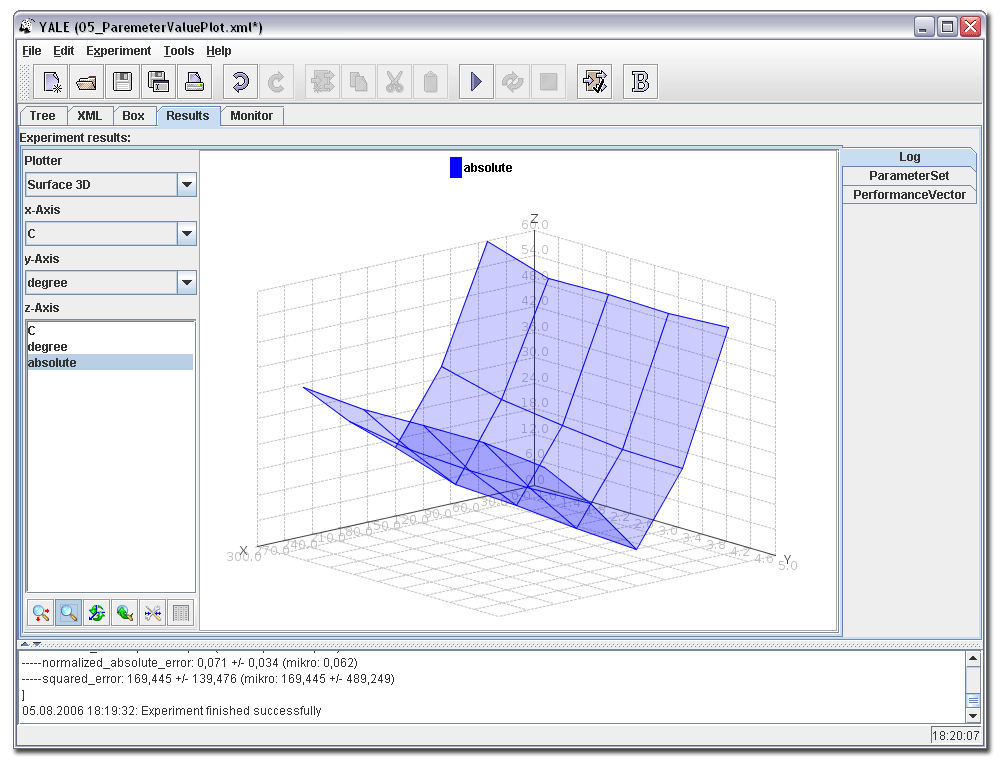
\includegraphics[height=0.4\textheight]{graphics/screenshots/screenshot_main2.png}
  \caption[Parameter optimization process screenshot]{\rapidminer screenshot of the continuous result display
    of a parameter optimization process.}
  \label{fig:screen_plot}
\end{figure}



\bigskip


Use \rapidminer and explore your data! Simplify the construction of data mining processes and
the evaluation of different approaches. Try to find the best combination of
preprocessing and learning steps or let \rapidminer do that automatically for
you. Have fun!




\section{How this tutorial is organized}

First you should read this chapter in order to get an idea of the concepts of
\rapidminer. Thereafter, we suggest that you read the GUI manual of \rapidminer
and make the online tutorial. It will be much easier to understand the
details explained in the next chapters. Chapter \ref{sec:first_steps}
describes possible first steps and the basics of \rapidminer. In Chapter
\ref{sec:advanced} we discuss more advanced processes. You should
read at least these two chapters to create your own
process setups. 
Chapter \ref{sec:operatorreference} provides information
about all \rapidminer core operators. It is an operator reference, i.e. you
can look up the details and description of all operators. 
Chapter \ref{sec:extending_rapidminer} can be omitted if you want to use
\rapidminer on your data or just want to perform some basic
process definitions. In this chapter we describe ways to extend \rapidminer by
writing your own operators or building own plugins.

